\subsection{M.PC.EAC - Estimated at Completion}

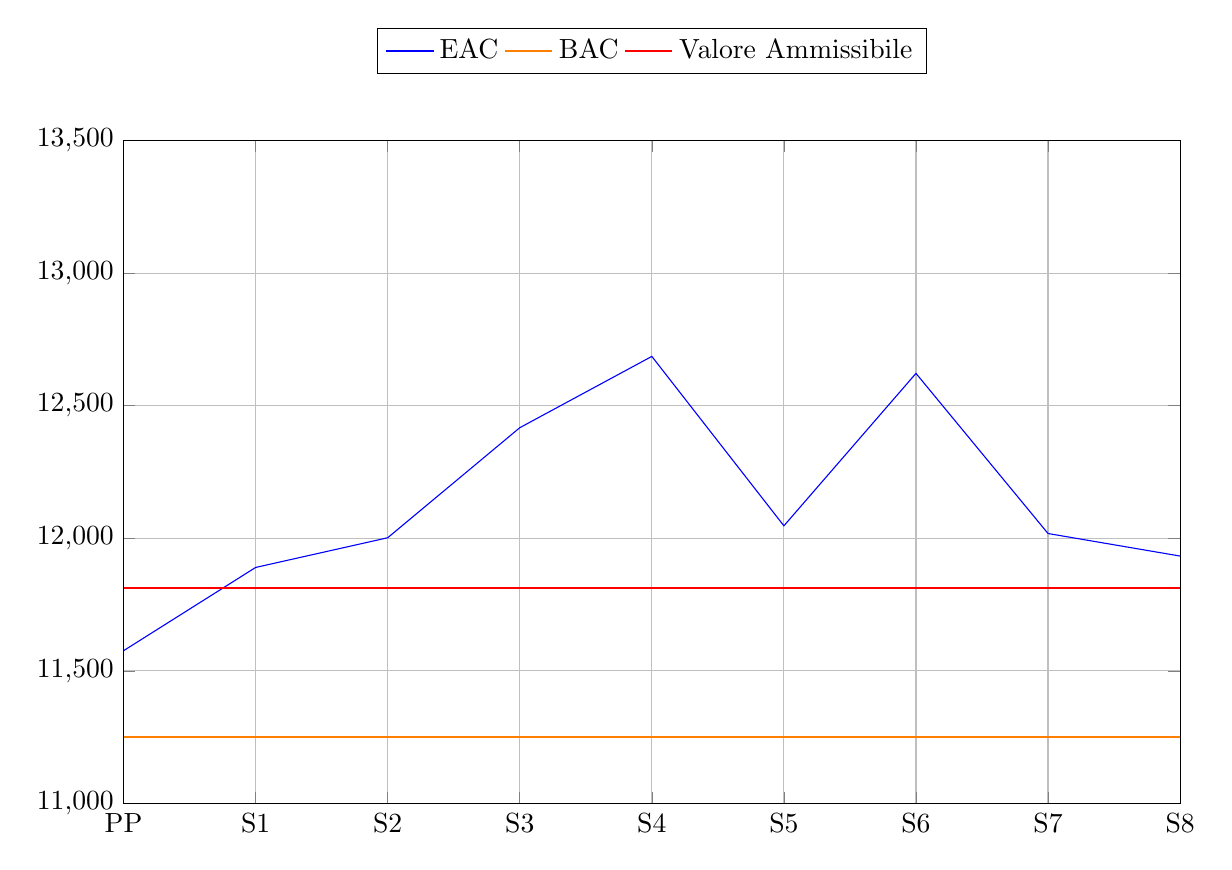
\begin{tikzpicture}
    \begin{axis}[
        width=15cm, height=10cm,
        ymin=11000, ymax=13500,
        xmin=0, xmax=8,
        xtick={0, 1, 2, 3, 4, 5, 6, 7, 8},
        xticklabels={ PP, S1, S2, S3, S4, S5, S6, S7, S8},
        xlabel={},
        ylabel={},
        grid=major,
        scaled ticks=false,
        legend style={at={(0.5,1.1)}, anchor=south, legend columns=-1},
    ]
    \addplot[color=blue] coordinates {(0, 11576) (1, 11890) (2, 12002) (3, 12417) (4, 12686) (5, 12047) (6, 12622) (7, 12018) (8, 11933) };
    \addlegendentry{EAC}
    \addplot[orange, thick] coordinates {(0, 11250) (8, 11250)};
    \addlegendentry{BAC}
    \addplot[red, thick] coordinates {(0, 11812.5) (8, 11812.5)};
    \addlegendentry{Valore Ammissibile}
    \end{axis}
\end{tikzpicture}
\subsubsection{RTB}
Il grafico mostra che l'\glossario{Estimated at Completion} non risulta mai all'interno del valore ammissibile, indicando una gestione poco efficiente dei costi di progetto. 
Questo significa che il costo stimato alla fine del progetto è sempre superiore al costo preventivato. Ciò indica che c'è necessità di un'analisi più approfondita dei costi e delle attività svolte per evitare ulteriori aumenti e per rientrare all'interno dei costi preventivati inizialmente.